\chapter[Accessible Area M]{Accessible Area (M), the BAM Framework, and Background Selection}

\begin{objetivos}
By the end of this chapter, readers should understand the accessible area
($M$); interpret the BAM framework; distinguish study, calibration, and
projection areas; delineate a biologically defensible $M$; generate background
points; compare biome-wide background with background restricted to $M$; and
prepare presence--background data for modeling \textit{Dinizia excelsa}.
\end{objetivos}

\section{Introduction}

Defining the accessible area, conventionally denoted by $M$, is one of the most
important decisions in species distribution modeling. It represents the portion
of geographic space historically accessible to a species through dispersal,
biogeographic history, landscape connectivity, and the absence of insurmountable
barriers \parencite{soberon2005,soberon2007,soberon2009,barve2011crucial}.

The definition of $M$ directly affects background selection, environmental
availability, contrasts between presences and absences or background, and hence
the parameters estimated by a model. An excessively broad $M$ may include
environments never accessible to the species; an overly restricted $M$ may
exclude gradients needed to estimate its niche.

\begin{conceito}[title={\faBook\quad Accessible area ($M$)}]
The accessible area is the set of regions a species could have reached during
its recent history, given dispersal, barriers, landscape connectivity, and
biogeographic history. It is not necessarily equivalent to the entire biome or
to the species' observed distribution.
\end{conceito}

\section{The BAM Framework}

The BAM framework describes species distributions through three components:
biotic factors ($B$), abiotic factors ($A$), and the dispersal-accessible area
($M$). In simplified terms, a species occurs where environmental conditions are
suitable, biotic interactions permit persistence, and the region has been
historically accessible.

\begin{equationbox}
\[
G_O = A \cap B \cap M
\]
Here, $G_O$ is the observed distribution, $A$ denotes suitable abiotic
conditions, $B$ denotes permissive biotic interactions, and $M$ is the
accessible area.
\end{equationbox}

\begin{atencao}[title={\faExclamationTriangle\quad The M area is not a technical detail}]
Defining $M$ changes the environmental conditions available to the model. The
choice must be biologically justified rather than based only on computational
convenience.
\end{atencao}

\section{Delineating M for \textit{Dinizia excelsa}}

Here, $M$ is operationally delineated from the final \textit{Dinizia excelsa}
records by buffering occurrences and restricting the result to the Amazon biome.
This reproducible didactic approach provides the foundation for subsequent
modeling chapters.

\rscriptfile{scripts/unidade05/01_estrutura_pastas.R}
\rscriptfile{scripts/unidade05/02_delimitar_area_m_dinizia.R}

\begin{figure}[H]
  \centering
  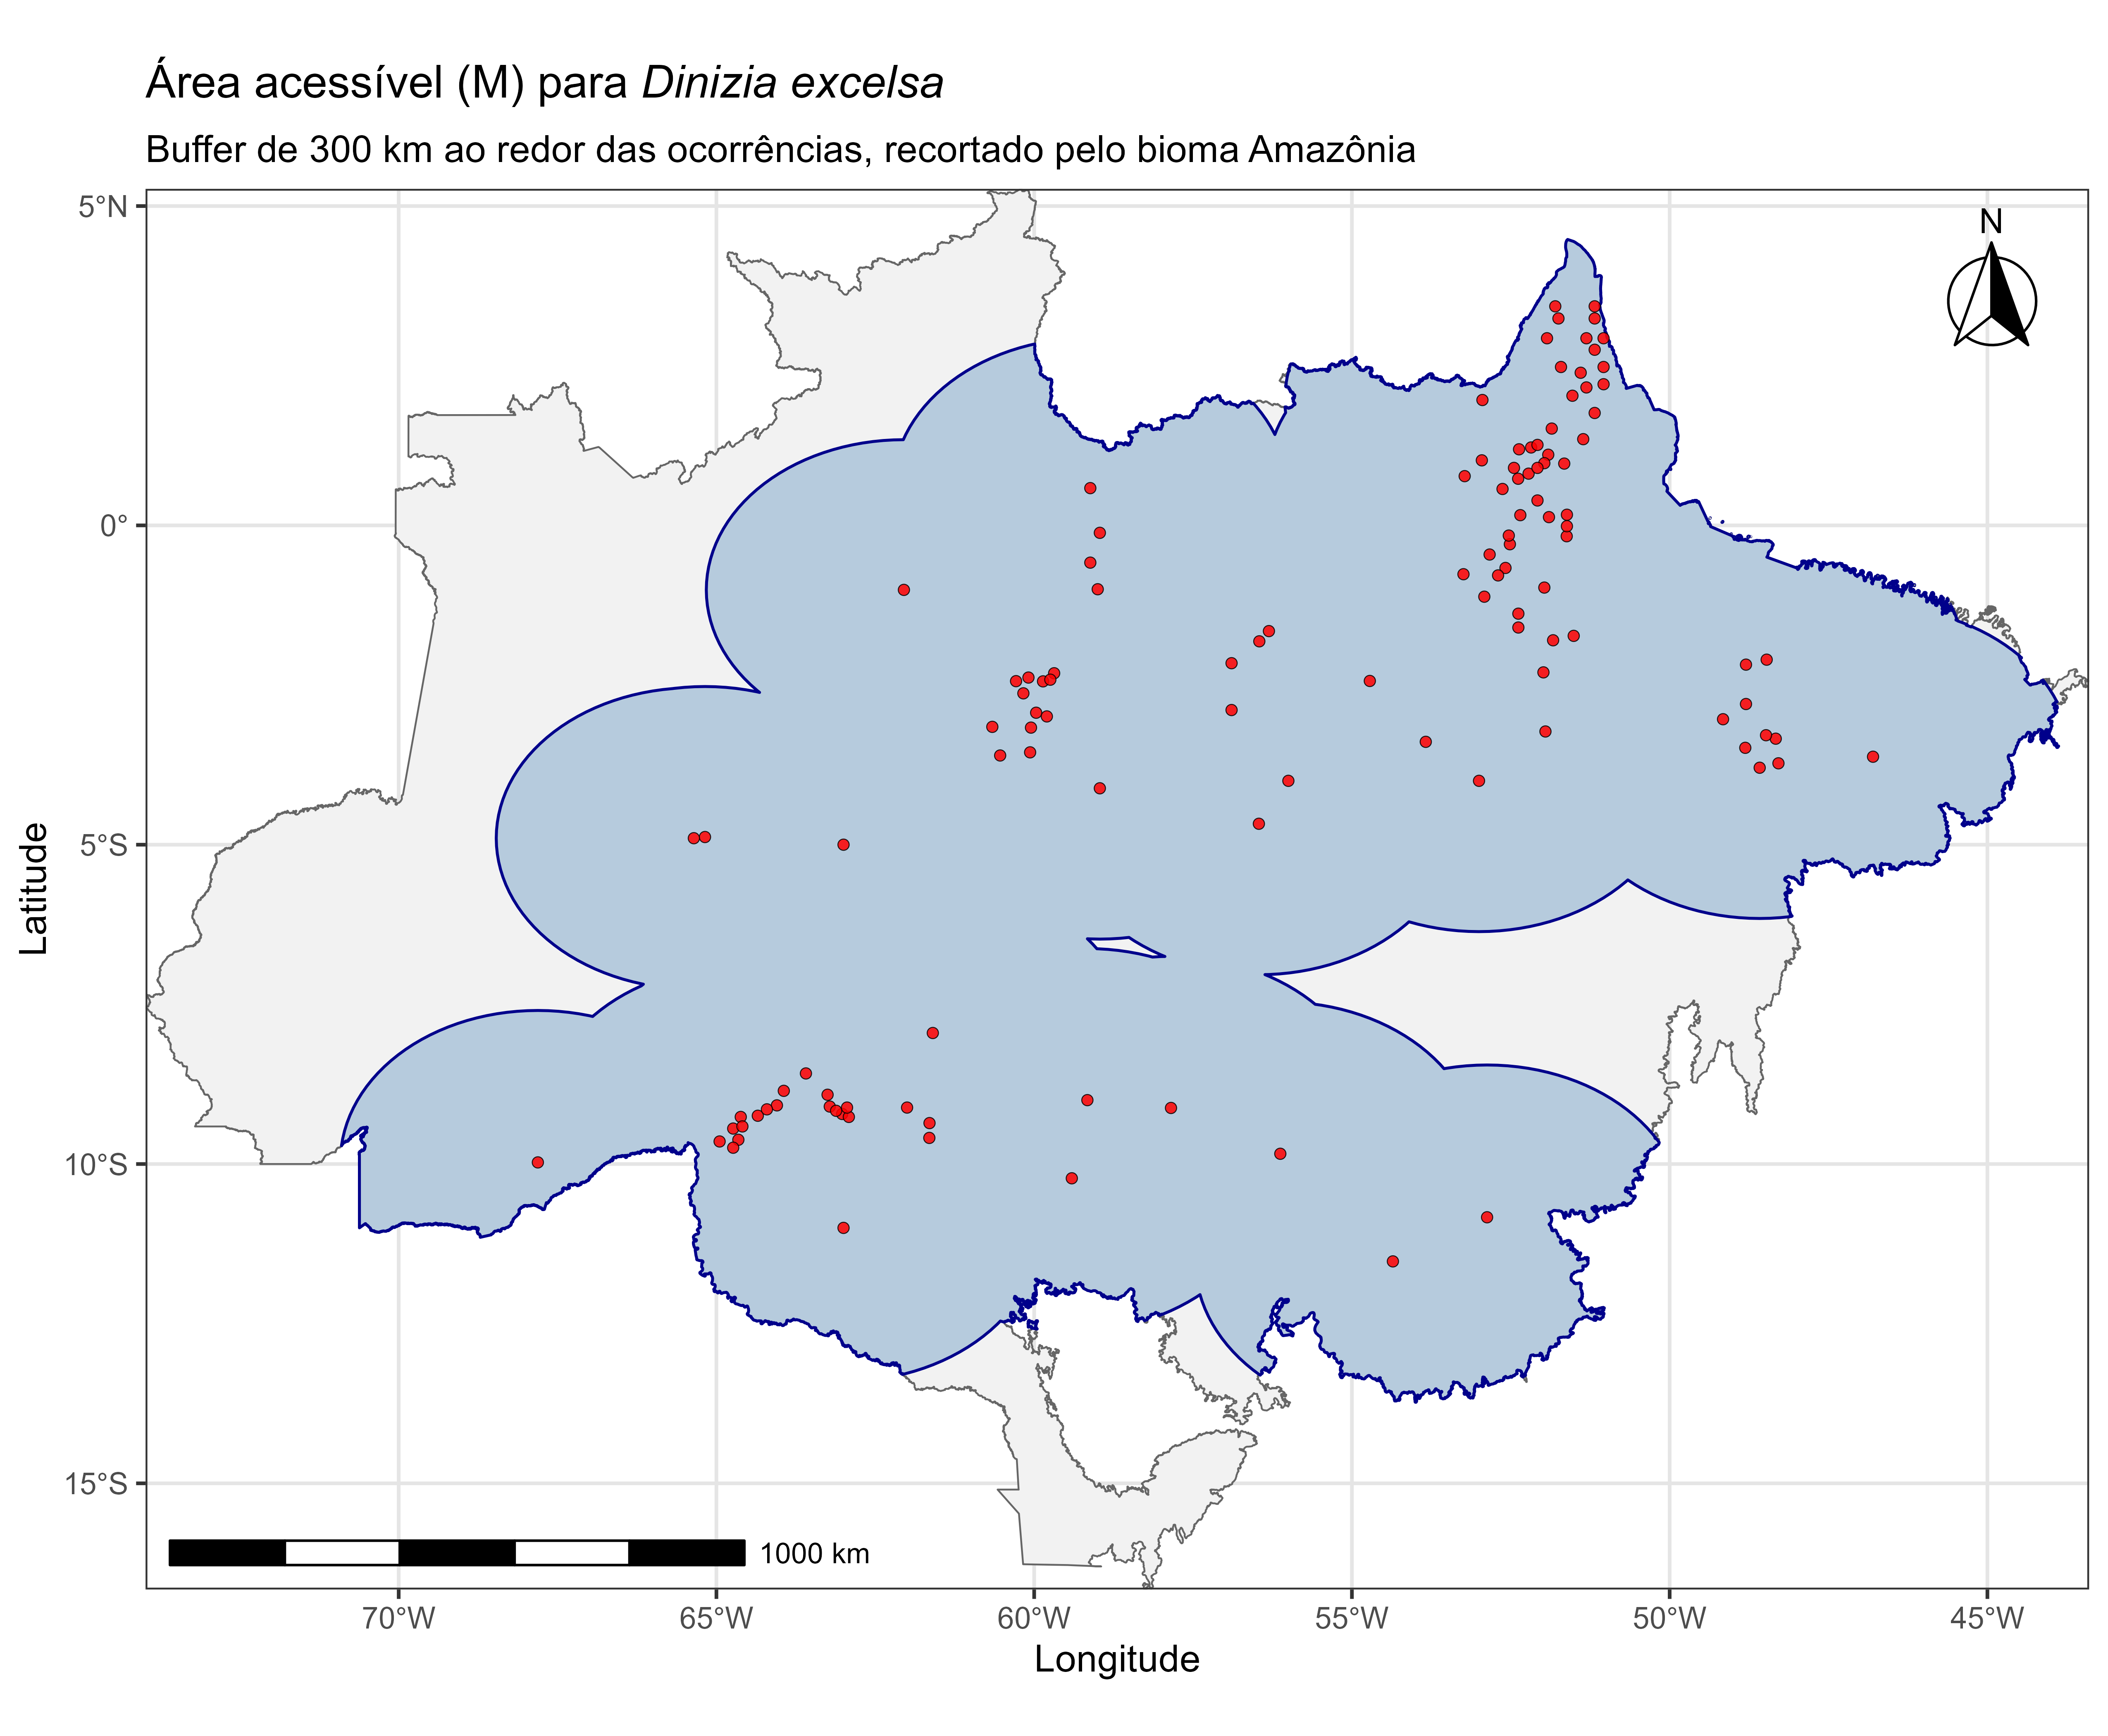
\includegraphics[width=0.90\textwidth]{figuras/unidade05/unidade05_area_m_dinizia.png}
  \caption{Accessible area ($M$) delineated for \textit{Dinizia excelsa} within the Amazon biome. The area was defined by buffering occurrences and cropping the result to the biome boundary.}
  \label{fig:unidade05_area_m_dinizia}
\end{figure}

\section{Background Selection}

Background points represent the environment available during model calibration.
They are not confirmed absences. They characterize environmental conditions
available within the area considered accessible.

\rscriptfile{scripts/unidade05/03_gerar_background_area_m.R}

\begin{figure}[H]
  \centering
  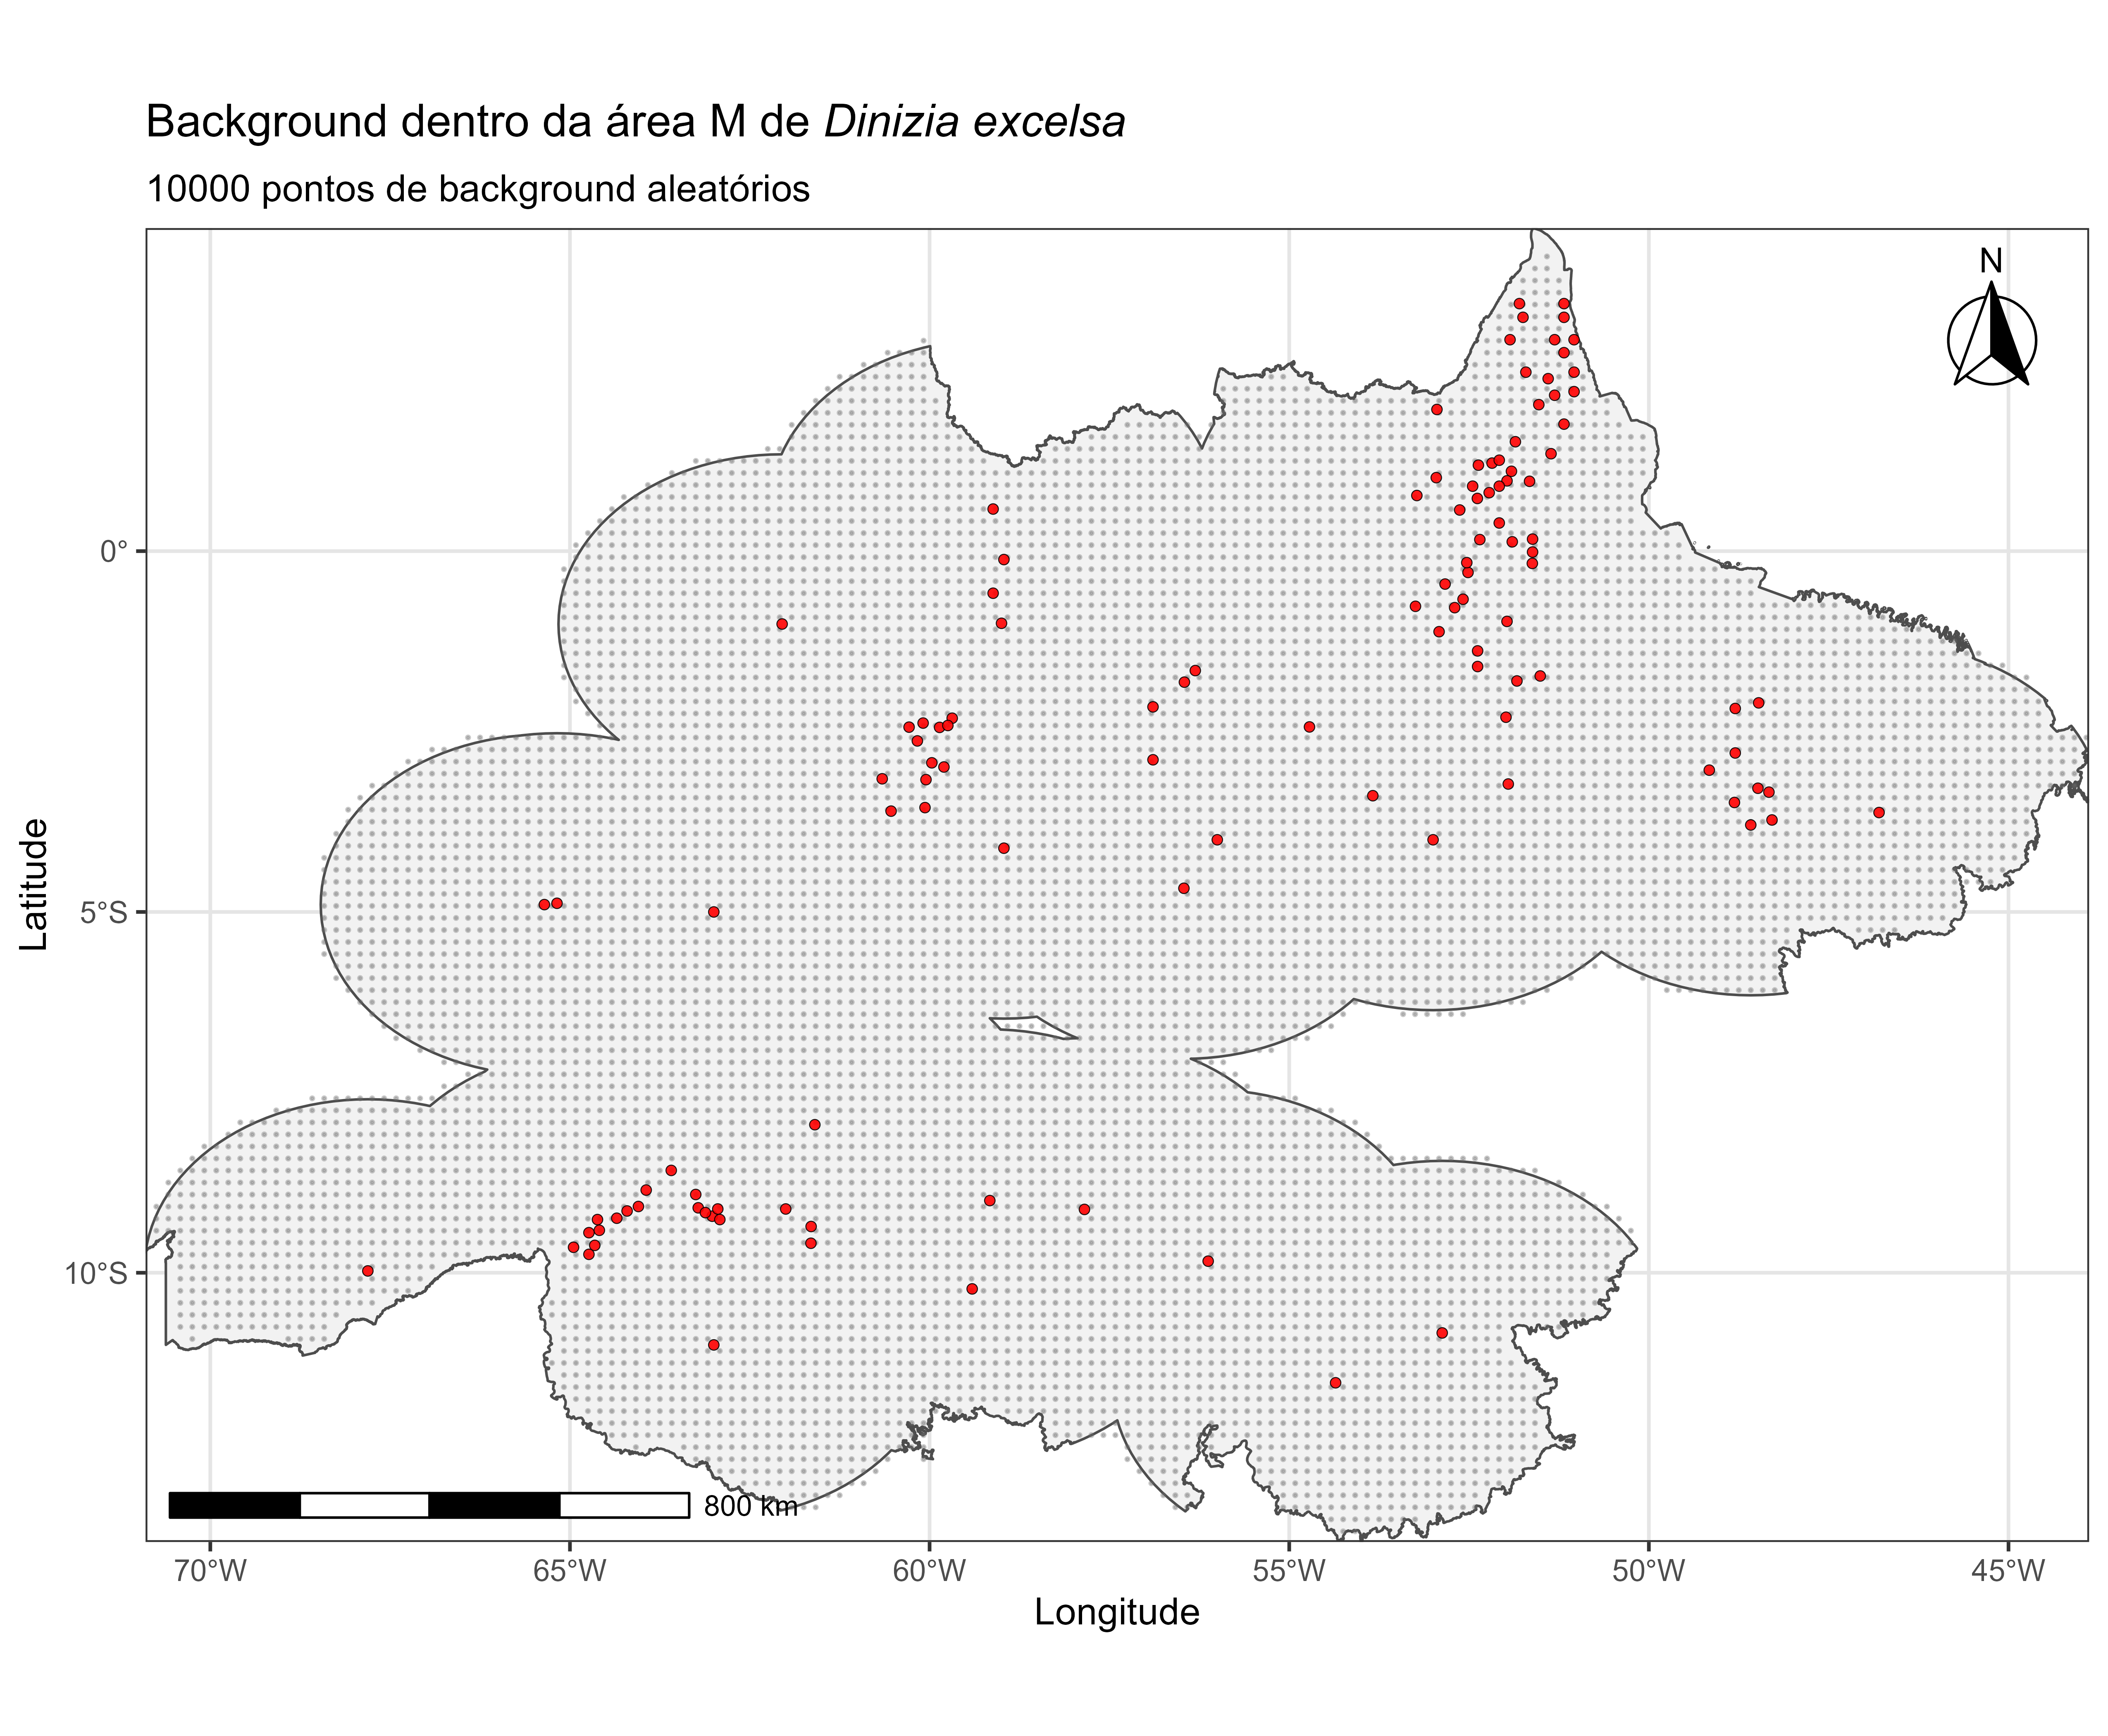
\includegraphics[width=0.90\textwidth]{figuras/unidade05/unidade05_background_area_m.png}
  \caption{Background points sampled within the accessible area ($M$) of \textit{Dinizia excelsa}.}
  \label{fig:unidade05_background_m}
\end{figure}

\section{Biome-Wide Background versus Background within M}

Background selection can substantially change the environmental distribution
available to a model. It is therefore informative to compare samples from the
entire biome with samples restricted to $M$.

\rscriptfile{scripts/unidade05/04_comparar_background_bioma_m.R}

\begin{figure}[H]
  \centering
  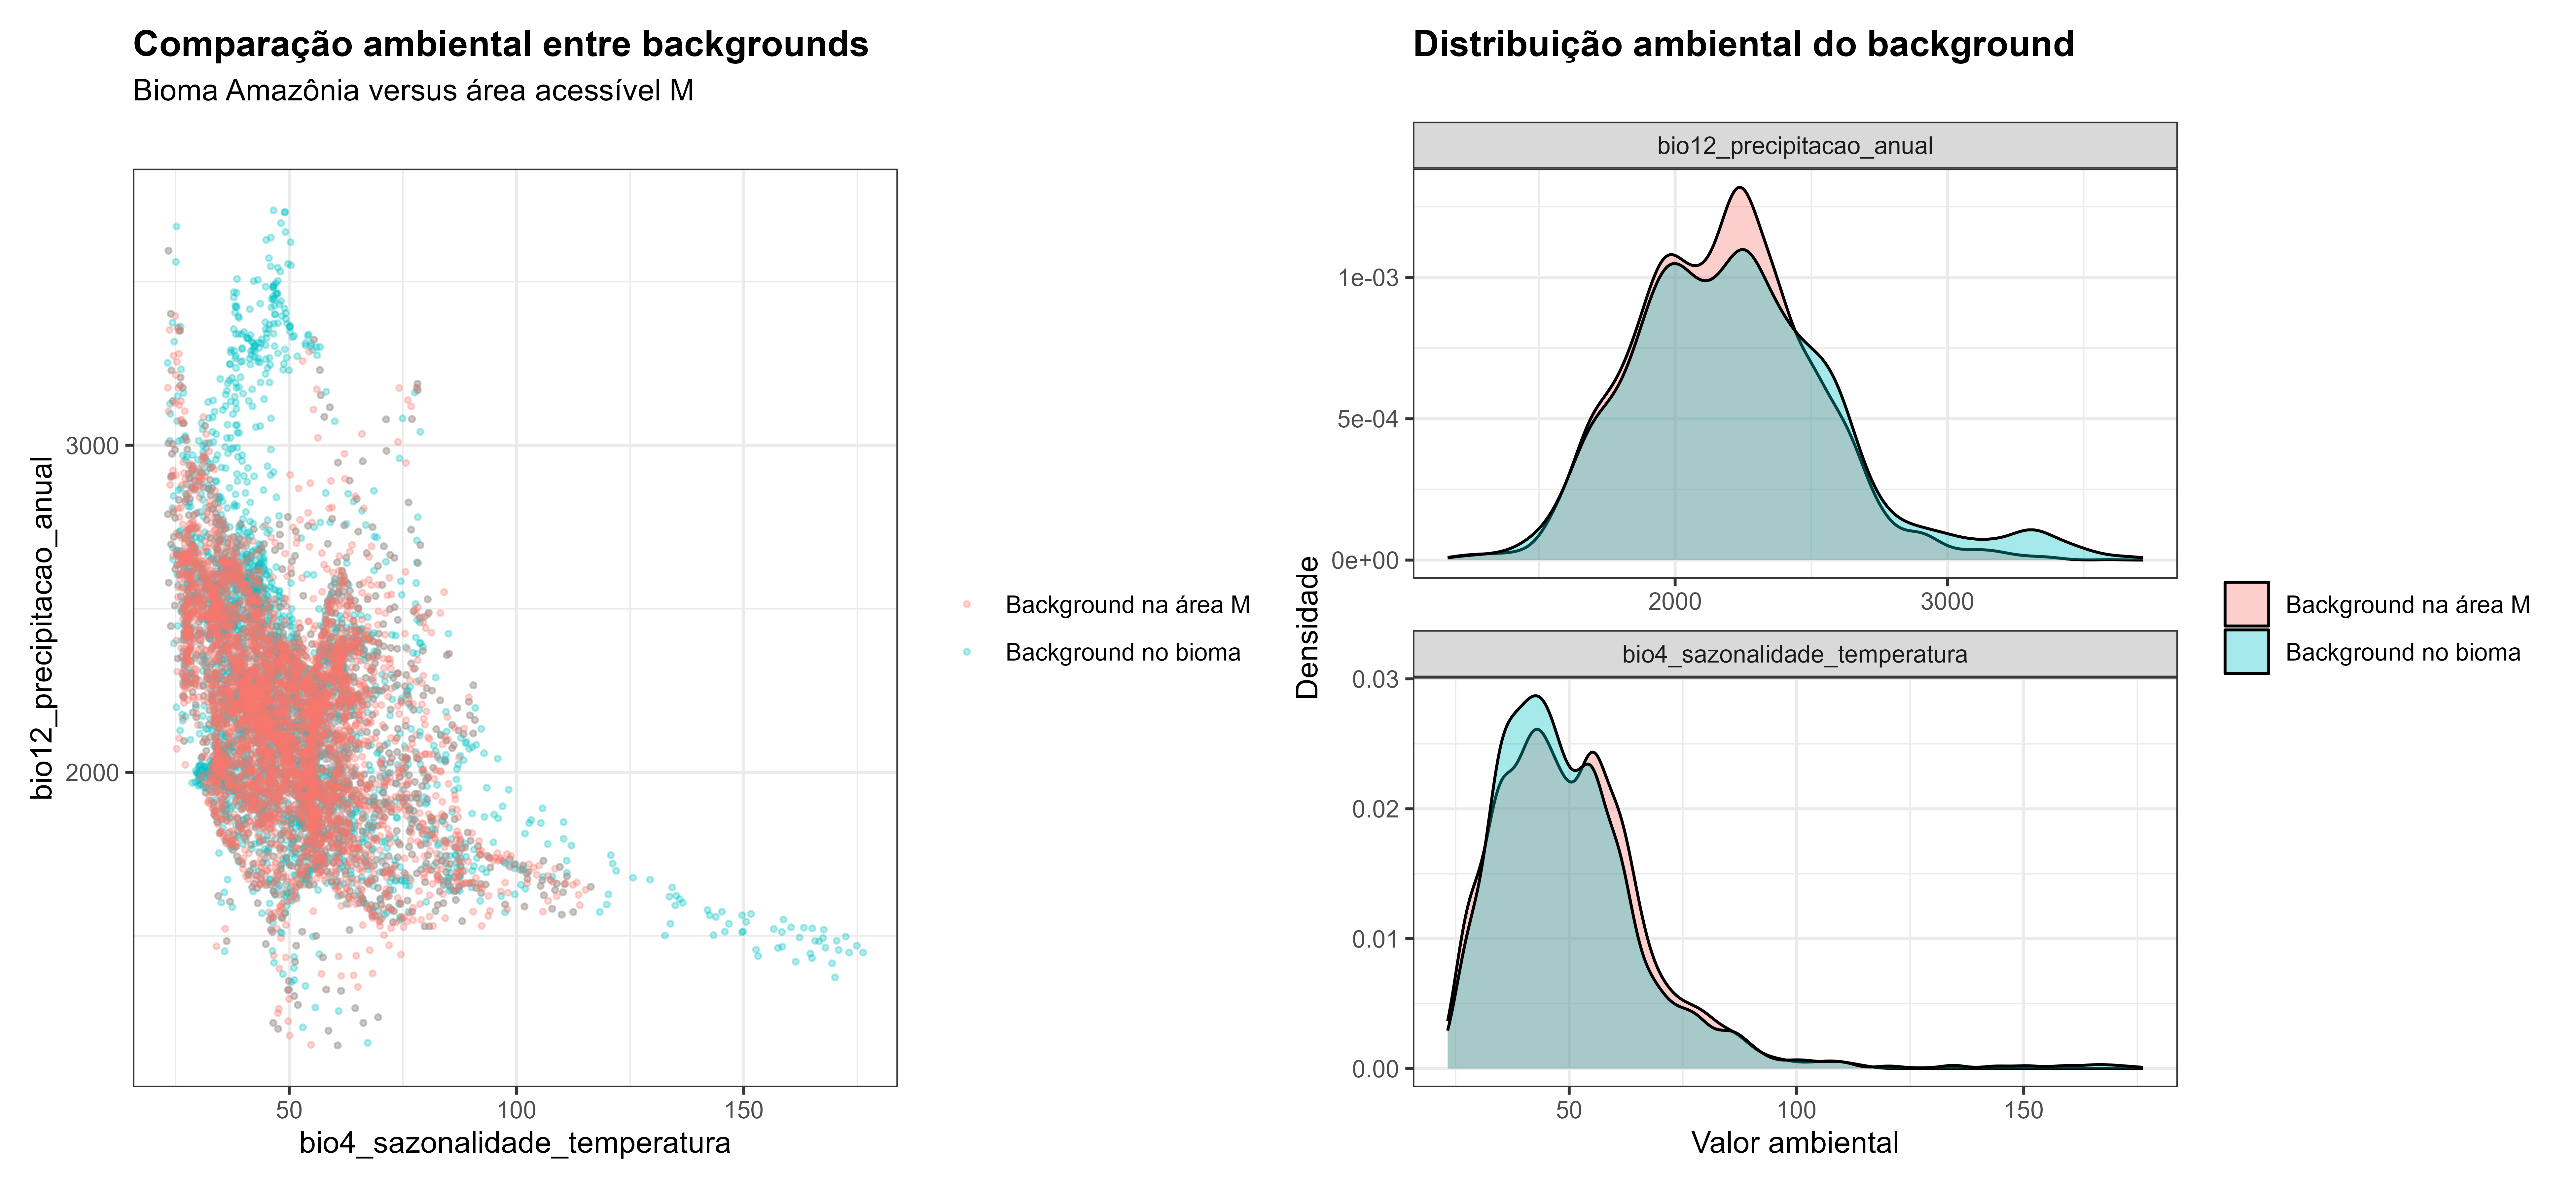
\includegraphics[width=0.90\textwidth]{figuras/unidade05/unidade05_comparacao_background.png}
  \caption{Comparison between background sampled throughout the Amazon biome and background restricted to the accessible area ($M$).}
  \label{fig:unidade05_comparacao_background}
\end{figure}

\section{Environmental Extraction and the Presence--Background Dataset}

The selected environmental variables are extracted at the presences and at
background points within $M$, producing the presence--background dataset used
in subsequent chapters.

\rscriptfile{scripts/unidade05/05_preparar_presenca_background.R}

\begin{figure}[H]
  \centering
  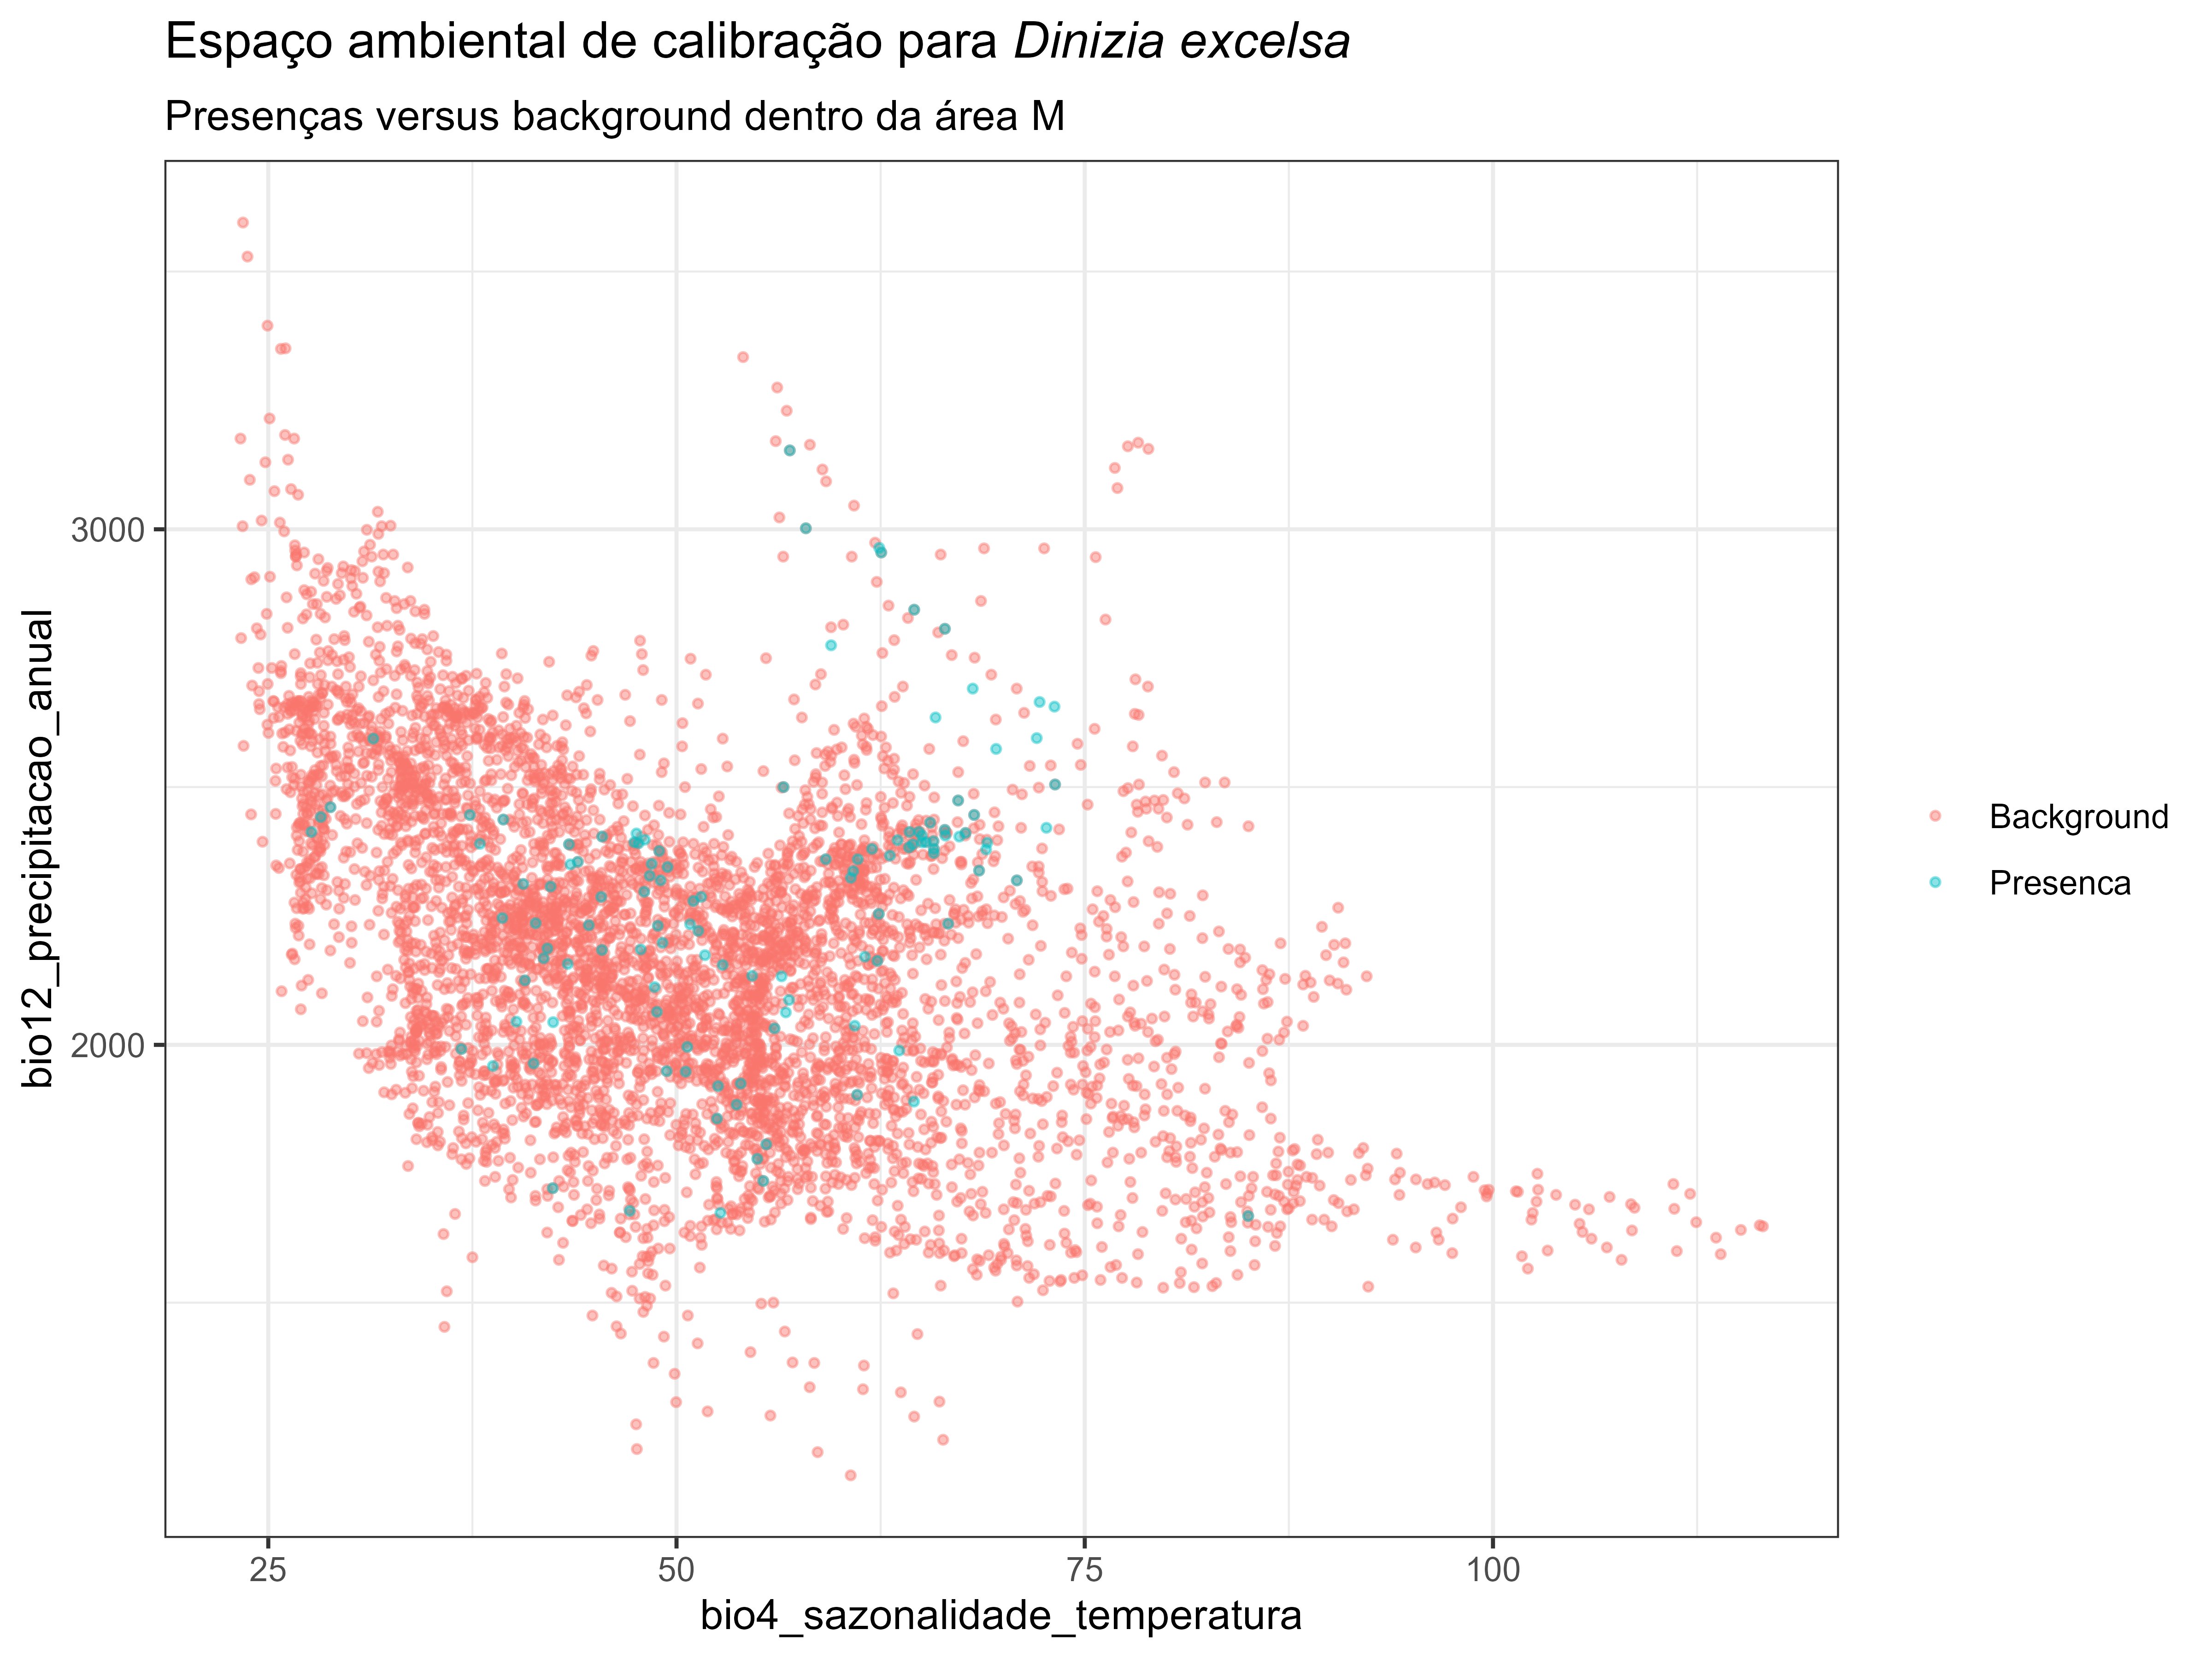
\includegraphics[width=0.86\textwidth]{figuras/unidade05/unidade05_espaco_ambiental_presenca_background.png}
  \caption{Environmental-space comparison between \textit{Dinizia excelsa} presences and background within the accessible area ($M$).}
  \label{fig:unidade05_espaco_presenca_background}
\end{figure}

\section{Complete Pipeline}
\rscriptfile{scripts/unidade05/06_pipeline_area_m_background.R}

\section{Chapter Summary}

Defining $M$ is an ecological, biogeographic, and methodological decision. It
affects model background, calibration, evaluation, and projection. The
operational $M$ delineated for \textit{Dinizia excelsa} provides a coherent
foundation for the models developed in the following chapters.

\begin{conceito}[title={\faBook\quad Key message}]
Background should represent the environment available to a species within its
accessible area. A model calibrated with inappropriate background can yield
biologically fragile maps even when statistical metrics appear strong.
\end{conceito}

